\documentclass{report}
\usepackage{graphicx}
\usepackage{float}
\usepackage{listings}
\usepackage{todonotes}
\usepackage[toc,page]{appendix}
%\usepackage[margin=1.5in]{geometry}

\begin{document}

\title{Virtual Power Plant design document}
\author{Ubbe Welling\\ubbe@eng.au.dk}

\maketitle

\setcounter{tocdepth}{2}
\tableofcontents

\chapter{Considerations and requirements}

\section{Overview}

The purpose of the Virtual Power Plant (VPP) platform is to:
\begin{itemize}
	\item receive measurements from sensors deployed in a building.
	\item receive current and forecast information from external sources on grid load, electricity price and more.
	\item process measurements and external information to make decisions on power usage.
	\item actuate devices deployed in a building to implement above mentioned decisions.
\end{itemize} 
The above functionality is already implemented in a number of individual applications and scripts. This system should provide the same functionality in an integrated application.

\section{Users and privileges}

\subsection{User categories}
An initial listing of envisioned users and their access to the system is shown below:

\paragraph{Residents}
\begin{itemize}
    \item{Actuate in own home}
    \item{See data from own home}
\end{itemize}

\paragraph{Janitor}
\begin{itemize}
    \item{Should be able to do anything he/she can already do before the system}
    \item{Actuate anything not in private}
    \item{Add/remove actuators}
\end{itemize}

\paragraph{Administrative staff (ie. housing association office staff)}
\begin{itemize}
    \item{See data on some level of aggregation. Maybe just reports?}
\end{itemize}

\paragraph{Aggregator}
\begin{itemize}
    \item{multiple buildings}
    \item{specific read/actuate permissions, granted by janitor/admin. staff}
\end{itemize}

\paragraph{System administrator}
\begin{itemize}
    \item{full access}
\end{itemize}

\subsection{Privileges requirements} \label{subsection:PrivilegesRequirements}
With outset in the above user categories and tasks, the following distinct privileges have been identified:

\paragraph{Global system privileges}
\begin{itemize}
    \item{Access to reports}
    \item{User access}
    \item{System admin access}
\end{itemize}

\paragraph{Building-specific privileges}
\begin{itemize}
    \item{Add new devices}
    \item{Remove devices}
\end{itemize}

\paragraph{Device-specific privileges}
\begin{itemize}
    \item{Read device status and data (measurements/actions)}
    \item{Configure device (configure parameters, disable)}
    \item{Remove device and data}
    \item{Actuate controller}
\end{itemize}

\chapter{Design}
The platform will consist of one main server application with an attached database. 

\section{Database design}
The database will reside in a PostgreSQL DBMS. 

\subsection{Schema: core}
The central part of the database schema is shown in figure \ref{figureDbCoreModel} and explained below:

\begin{figure}[H]
    \centering
    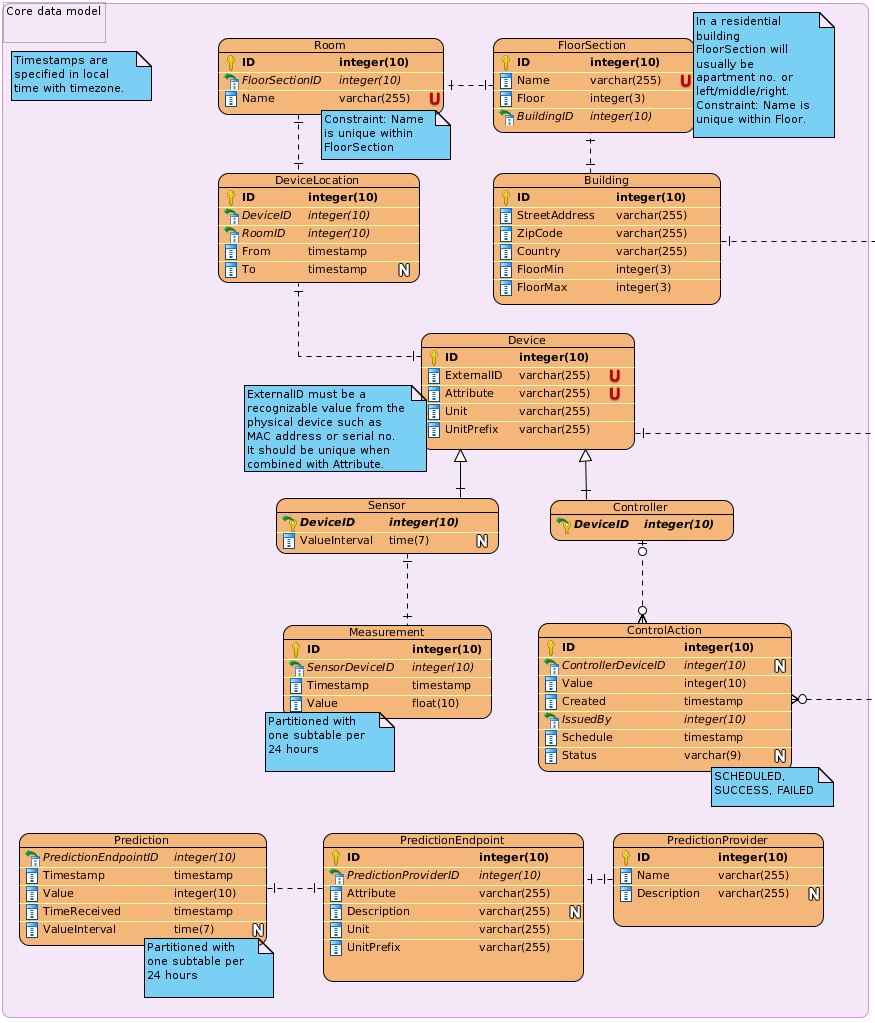
\includegraphics[width=\textwidth]{figures/db_core_schema}
    \caption{Database core schema}
    \label{figureDbCoreModel}
\end{figure}

\subsubsection{Devices and measurements}

\paragraph{Device} 
Entries in \texttt{Device} correspond to physical control and sensor devices, with the modification that we store one logical device for each function of the physical device. Whether a device is a sensor or a controller is specified by its presence in table \texttt{Controller} or \texttt{Sensor}. Columns \texttt{Attribute},\texttt{Unit} and \texttt{UnitPrefix} (such as milli) are for sensors specification of the incoming measurement values, while they for controllers specify the format of values to send to the controller when actuating it.

\paragraph{Sensor} 
Table \texttt{Sensor} specifies an optional property \texttt{ValueInterval} which is used when values are aggregated over a limited time interval (such as 15 minutes). 

\paragraph{Measurement} 
This table will contain a row for each measurement received from a physical sensor. It will simply consist of a \texttt{Value}, a \texttt{Timestamp} and a reference into \texttt{Sensor}, which enables interpretation of the value. The \texttt{Measurement} table is expected to grow very large and will therefore be partitioned into subtables that will each contain 24 hours of measurements and can be discarded on the fly according to the rolling window strategy explained in section \ref{subsection:rollingwindow}.

\paragraph{ControlAction} 
Table \texttt{ControlAction} will contain scheduled and past commands for controllers. An action is simply specified by a \texttt{Value} which can be interpreted via the reference into table \texttt{Controller} and \texttt{Device}. Column \texttt{Schedule} specifies the time for carrying out the action, and \texttt{Status} indicates if execution is still pending or has been completed. Finally, \texttt{IssuedBy} specifies which user scheduled the action. We might consider partitioning and discarding of old data in this table in the same way as for table \texttt{Measurement}.

\paragraph{Building, FloorSection, Room}
The physical properties of a building are modeled in these tables. A building consists of an integer range of floors. Each floor consists of \texttt{FloorSection}s which in most cases will be equivalent to apartments. The generalized term FloorSection is intended to support other types of buildings where designations such as "South wing" or other may be desired. Finally, a floor consists of named \texttt{Room}s. We do not expect to obtain device locations with a higher degree of accuracy than individual rooms.

\paragraph{DeviceLocation} This table maps \texttt{Device}s to \texttt{Room}s for specified time periods, indicating that devices may be moved around.

\subsubsection{Predictions}
Predictions of a wide range of values (power consumption, grid load, price, CO\textsubscript{2} emissions, ...) will be received from external data providers and will in addition be generated by our own application logic. 

While the data stored for predictions is quite similar to those for measurements, we have chosen to store them separately because of the fundamentally different semantics.

\paragraph{PredictionProvider}
An entity providing predictions, such as energinet.dk or the system itself.

\paragraph{PredictionEndpoint} 
A logical source of predictions of one type. Specifies the \texttt{Attribute},\texttt{Unit} and \texttt{UnitPrefix} of the incoming values and provides an optional \texttt{Description}.

\paragraph{Prediction}
Actual prediction values. \texttt{Timestamp} indicates the time for which the value applies, while \texttt{TimeReceived} indicated when the prediction was received from the provider. This is relevant since multiple predictions for the same future point in time may be received over time. Some values actually cover an interval (for instance predicted power consumption for a given day of 24 hours), which is specified in column \texttt{ValueInterval}.
This table is also expected to grow quickly, motivating the same partitioning and rolling window strategy as for table \texttt{Measurement}.

\subsection{Schema: Users, groups and privileges}

The database schema for storing users and privileges has been developed to meet the requirements from section \ref{subsection:PrivilegesRequirements}. This is shown below:

\begin{figure}[H]
    \centering
    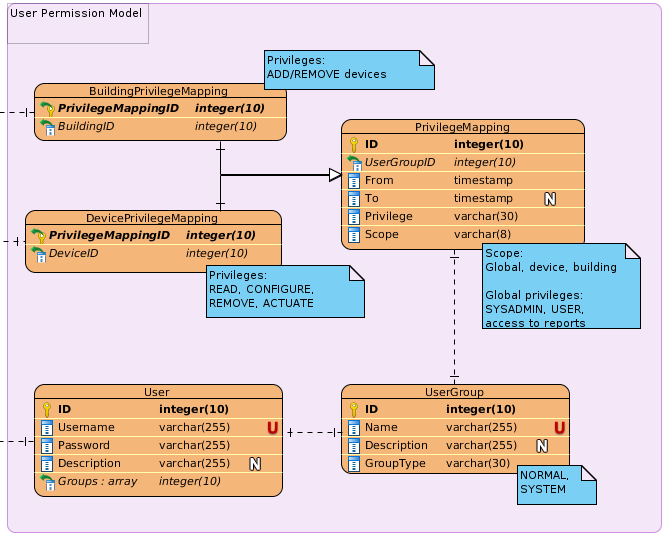
\includegraphics[width=\textwidth]{figures/db_user_schema}
    \caption{Users and privilege schema}
\end{figure}

\paragraph{Users and UserGroups}
\texttt{User}s have a username and a password (which will be hashed with a suitable one-way hash function) and can be member of a number of \texttt{UserGroup}s. 

\paragraph{PrivilegeMapping}
This table maps \texttt{UserGroup}s to specific privileges. A mapping includes a time period which may be open-ended. In order to have privileges for specific devices and buildings as well as globally valid ones, a \texttt{Scope} must be set. In case of a device or building-specific privilege, the concerned \texttt{Device} or \texttt{Building} must be looked up in \texttt{DevicePrivilegeMapping} or \texttt{BuildingPrivilegeMapping} respectively. These tables are intended to have corresponding subtypes in the object-oriented implementation.

It will be up to application logic to interpret the semantics of the concrete privileges.

\subsection{Subject to change}
We can already foresee that configuration of controllers as well as other settings will most likely require extensions to the above proposed schema. The basic structure of the core schema should however not change.

\subsection{Rolling window}\label{subsection:rollingwindow}
Since the \texttt{Measurement} table will grow very quickly, a the partitioning and data discarding scheme will be employed. The table will be partitioned in time intervald, having one subtable for every 24 hours. Furthermore, subtables older than one week will be dropped. The time limits can naturally be configured. The same scheme might be applied to tables \texttt{ControlAction} and \texttt{Prediction}.
This done in order to accomodate the VPP application on a desktop size machine with limited disk space.

\subsection{Data warehouse}
In order to retain data, the VPP will periodically forward data to an external database (data warehouse) that can accomodate a larger volume of data for longer periods. When forwarding data, measurements may be averaged over limited time intervals to reduce data size. The data warehouse can then be used for statistics and historical analysis. While the data warehouse schema was initially planned to be identical to the VPP rolling window DB, the presence of users, privileges and most likely various other configuration indicates that probably only the core schema as shown in figure \ref{figureDbCoreModel} should be present in the data warehouse. 

\section{Application design}
The application will be programmed in object-oriented Python, using Python processes to enable concurrent processing.

Key classes have been identified to form a static structure which is shown in figure \ref{figureClassDiagram} and elaborated below:

\begin{figure}[H]
    \centering
    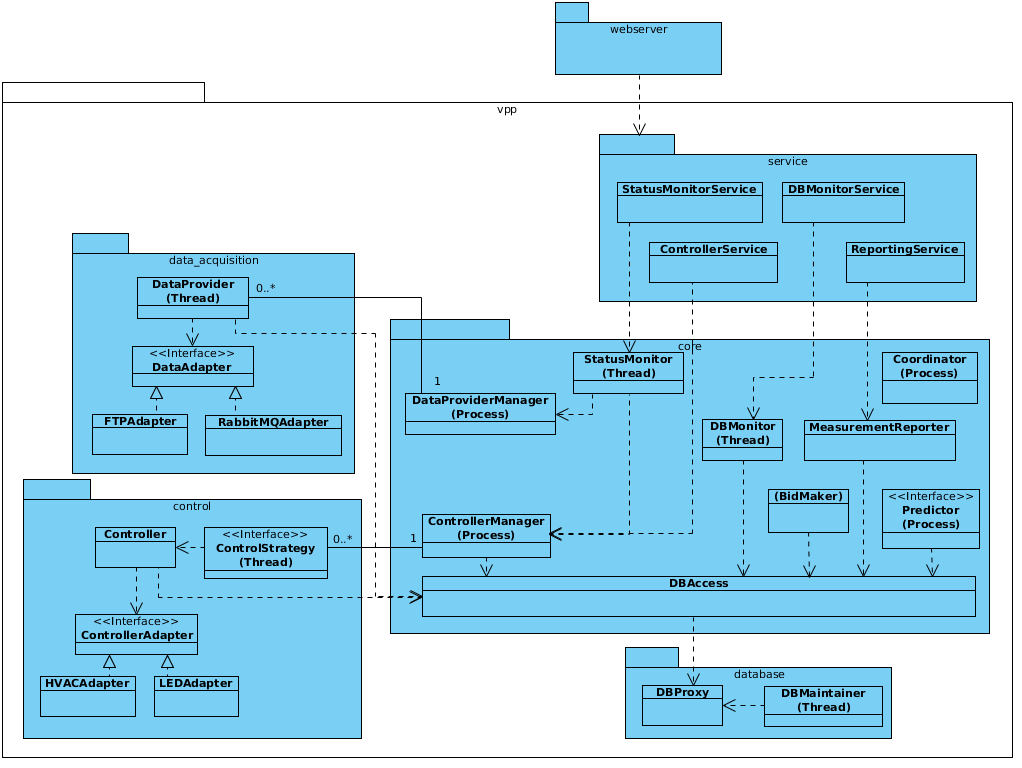
\includegraphics[width=\textwidth]{figures/class_diagram}
    \caption{Class diagram}
    \label{figureClassDiagram}
\end{figure}




%\begin{appendices}


\end{appendices}



\end{document}